\documentclass[a4paper,12pt]{report}
\addtolength{\oddsidemargin}{-1.cm}
\addtolength{\textwidth}{2cm}
\addtolength{\topmargin}{-2cm}
\addtolength{\textheight}{3.5cm}
\newcommand{\HRule}{\rule{\linewidth}{0.5mm}}
\makeindex

\usepackage{longtable}
\usepackage{graphicx}
\usepackage{makeidx}
\usepackage{hyperref}
\usepackage{verbatim}

\hypersetup{
    colorlinks=true,
    linkcolor=blue,
    filecolor=magenta,      
    urlcolor=cyan,
}


% define the title
\author{Ambitious Design}
\title{ Software Requirements Specifications and Technology Neutral Process Design}
\begin{document}
\setlength{\parskip}{6pt}

% generates the title
\begin{titlepage}

\begin{center}
% Upper part of the page           
\textsc{\LARGE Department of Computer Science}\\[1.5cm]
\textsc{\Large COS 301 - Main Project}\\[0.5cm]
% Title
\HRule \\[0.4cm]
{ \huge \bfseries Document 1}\\[0.4cm]
\HRule \\[0.4cm]
% Author and supervisor
\begin{minipage}{0.4\textwidth}
\begin{flushleft} \large
\emph{Author:}\\
Tim {Kirker}
\end{flushleft}
\end{minipage}
\begin{minipage}{0.4\textwidth}
\begin{flushright} \large
\emph{Student number:} \\
u11152402
\end{flushright}
\end{minipage}
\begin{minipage}{0.4\textwidth}
\begin{flushleft} \large
\emph{} \\
Stephen {Swanepoel}
\end{flushleft}
\end{minipage}
\begin{minipage}{0.4\textwidth}
\begin{flushright} \large
\emph{} \\
u11032091
\end{flushright}
\end{minipage}
\begin{minipage}{0.4\textwidth}
\begin{flushleft} \large
Dian {Veldsman}
\end{flushleft}
\end{minipage}
\begin{minipage}{0.4\textwidth}
\begin{flushright} \large
\emph{} \\
u12081095
\end{flushright}
\end{minipage}
\begin{minipage}{0.4\textwidth}
\begin{flushleft} \large
Killian {Kieck}
\end{flushleft}
\end{minipage}
\begin{minipage}{0.4\textwidth}
\begin{flushright} \large
\emph{} \\
u12252213
\end{flushright}
\end{minipage}


{\large \today}
\end{center}
\end{titlepage}
\footnotesize
\normalsize

\renewcommand{\thesection}{\arabic{section}}
\newpage
\begin{center}
\textsc{\LARGE Software Requirements Specification}\\[1.5cm]
\end{center}



\section{Introduction}
This document aims to set out the functional and non-functional requirements of a system as specified by the Willburg Outdoor PTY(ltd.). The system is required to assess an image by sorting the image into baskets and groupings and then identify if a human is present in the picture. The document will also serve the purpose of communicating the requirements and specifications as needed by the client.

 \subsubsection{Vision}
 The client for this project, Willburg Outdoor PTY(ltd.), has called for the design of an application that will assess an images, identify a human(s) in the image. If a human has been identified by the system, a call must then be set out to warn a user. The main idea behind the project is to be able to alert the user, of the Willburg camera, that a human has been identified so that the user will be informed about the movement around the camera.

\subsubsection{Background}
Rhino poaching is currently at a crisis point. By the end of 2015, the number of African rhinos killed by poachers had increased for the sixth year in a row with at least 1,338 rhinos killed by poachers across Africa in 2015. South Africa has by far the largest population of rhinos in the world and is an incredibly important country for rhino conservation. However rhino poaching levels have dramatically escalated over recent years. \\
\\The South African farm attacks are an ongoing trend of violent attacks on farmers in South Africa. Between 1994 and March 2012, there have been 361,015 murders in South Africa. While the police are supposed to regularly visit commercial farms to ensure security, they claim they cannot provide effective protection due to the wide areas that need to be covered and a lack of funding.\\
\\Willburg Outdoor is company that is passionate about the South Africa. With this passion comes the need to protect its farmers and it animals from those who intend to harm them.The client intends to use the system to fight these two problems by alerting the user of the Willburg camera of the identification in an effort to potentially stop a crime or poaching from accuring. This will hopefully deter future poachers and farm attackers.
	
\section{Architecture Requirements}
\subsection{Access Channel Requirements}
Any and all interactions by the user will be done through the Willburg Application.
\subsection{Quality Requirements}
\subsubsection{Performance}
\begin{enumerate}
	\item Images should only be captured and processed if some movement is detected to ensure that the server does not get overloaded.
	\item Images which are processed should not be large in size so they may be processed faster by the server.
	\item The system must be created with the most minimal and efficient coding
	practices possible, given that the result must still be reliable and robust.
\end{enumerate}
\subsubsection{Reliability}
\begin{enumerate}
	\item The system must be thoroughly tested on the server side, to
	ensure it will not cause faults or problems. 
	\item The notification warning users will receive must be sent out immediately after the image has been processed in a real-time manner.
\end{enumerate}
\subsubsection{Scalability}
\begin{enumerate}
	\item Modular programming should be used in order to ensure that there are no restrictions in terms of the systems ability to be extended and improved upon at later stages.
	\item The server should be able to process multiple images at once to ensure the real-time restriction is met.
\end{enumerate}
\subsubsection{Security}
\begin{enumerate}
	\item Depending on the technology being used the various security measures should be in place to ensure the integrity of the server, such as: SQL injections etc.
\end{enumerate}
\subsubsection{Flexibility}
\begin{enumerate}
	\item The system should be able to perform correctly even while under strain due to bulk processing without any loss of data.
	\item The system should be modularized to ensure both easy testing of components as well as addition of components without affecting the system.
\end{enumerate}
\subsubsection{Maintainability}
\begin{enumerate}
	\item The system should be designed in technologies which offer user support and continuous updates for extra functionality.
	\item The system must be well structured and documented to ensure future developers are able to understand and maintain the system.
	\item The modular design of the system must be such that if changes must be made to a part of the system, only that part itself should be changed.
\end{enumerate}
\subsubsection{Auditability}
\begin{enumerate}
	\item All images processed should be logged and traceable(user, date, time etc.) once pushed into the database.
\end{enumerate}
\subsubsection{Integrability}
\begin{enumerate}
	\item The system should be designed in a manner which allows for easy 
\end{enumerate}
\subsubsection{Cost}
\begin{enumerate}
	\item The tools used to design the system should, as far as possible be open source, free and not require a license.
	\item In certain cases, paid and licensed software may be suitable for specific aspects of the system. 
\end{enumerate}
\subsubsection{Usability}
\begin{enumerate}
	\item The Willburg application should be easy for users to interact with regarding the notifications they will be receiving.
\end{enumerate}
\newpage
 \subsubsection{Integration Requirements}
 The following are the integration requirements for the Smart Image Identifier project:
 	\begin{itemize}
 		\item Integration channels The main integration channel that will be used for this project is Javascipt. This will allow us to communicate with their temporary server that contains all the images we will be using for the project.
 	\end{itemize}
	\begin{itemize}
 		\item Protocols
	\end{itemize}
	\begin{itemize}
 		\item API specifications
	\end{itemize}
	\begin{itemize}
 		\item Quality requirements
			\begin{itemize}
				\item Performance: The performance for the integration is important, such that the sooner a human is identified the sooner measures can be taken. How ever we are limited to the speed of the camera transmitters and thus will focus on notifying the client as fast as we can as opposed to sending the image.
				\item Scalability: The clients will maintain their image servers so that they may take and store as many images as necessary. The application that will be used by the customers will be available through the app store and will allow for a large customer base to download it.
				\item Security: The clients picture servers must be completely secure as they contain incredibly sensitive data.
			\end{itemize}
	\end{itemize}
	
 \subsubsection{Architecture Constraints}
	Technologies to be used:
		\begin{itemize}
			\item OpenCv
			\\
		\end{itemize}
\newpage
\section{Functional Requirements and Application Design}
\subsection{Use Case Prioritisation}
	\begin{itemize}
		\item[$\bullet$]\textbf{Set Search Target}\newline

		\textbf{Description:} A person with access to software can set the what the smart image identifier must search for.\newline
		
		\textbf{Use Case Prioritisation:} Nice-To-Have\newline

		\textbf{Pre-Conditions:}
		\begin{itemize}
			\item[$\bullet$]Administrator must enter valid criteria to search for.
			\\
		\end{itemize}
		\textbf{Post-Conditions: }
		\begin{itemize}
			\item[$\bullet$]Administrator can see what the Smart Image Identifier is searching for.
			\\
		\end{itemize}
		\item[$\bullet$]\textbf{Create Table}\newline

		\textbf{Description:} Create new tables in the database to categorize the data into baskets.\newline
		
		\textbf{Use Case Prioritisation:} Critical\newline
		
		\textbf{Pre-Conditions:}
		\begin{itemize}
			\item[$\bullet$]System must have access to the database.
			\\
		\end{itemize}
		\textbf{Post-Conditions: }
		\begin{itemize}
			\item[$\bullet$]New database table is created.
			\\
		\end{itemize}
		\newpage
		\item[$\bullet$]\textbf{Insert Data}\newline

		\textbf{Description:} Move images (data) in the database from one table to another.\newline
		
		\textbf{Use Case Prioritisation:} Critical\newline

		\textbf{Pre-Conditions:}
		\begin{itemize}
			\item[$\bullet$]System must have access to the database.
			\item[$\bullet$]Table must exist.
			\\
		\end{itemize}
		\textbf{Post-Conditions: }
		\begin{itemize}
			\item[$\bullet$]Image is moved to selected table.
			\\
		\end{itemize}
		\item[$\bullet$]\textbf{Retrieve Data}\newline

		\textbf{Description:} Retrieve images (data) from the database to be analyzed.\newline
		
		\textbf{Use Case Prioritisation:} Critical\newline

		\textbf{Pre-Conditions:}
		\begin{itemize}
			\item[$\bullet$]System must have access to the database.
			\item[$\bullet$]Image(data) being retrieved must be in the database.
			\\
		\end{itemize}
		\textbf{Post-Conditions: }
		\begin{itemize}
			\item[$\bullet$]Image(data) is still inside the database.
			\\
		\end{itemize}
		\newpage
		\item[$\bullet$]\textbf{Delete Data}\newline

		\textbf{Description:} Removes images (data) from the database.\newline
		
		\textbf{Use Case Prioritisation:} Important\newline

		\textbf{Pre-Conditions:}
		\begin{itemize}
			\item[$\bullet$]System must have access to the database.
			\item[$\bullet$]Image(data) to be deleted must be in the database.
			\\
		\end{itemize}
		\textbf{Post-Conditions: }
		\begin{itemize}
			\item[$\bullet$]Image(data) is removed from the database.
			\\
		\end{itemize}
		\item[$\bullet$]\textbf{Alert}\newline

		\textbf{Description:} Alert the user when an image being searched contains the search criteria in it.\newline
		
		\textbf{Use Case Prioritisation:} Critical\newline

		\textbf{Pre-Conditions:}
		\begin{itemize}
			\item[$\bullet$]Image(data) must contain the search criteria in it.
			\\
		\end{itemize}
		\textbf{Post-Conditions: }
		\begin{itemize}
			\item[$\bullet$]User is alerted.
			\item[$\bullet$]Image(data) is included with the alert.
			\\
		\end{itemize}
	\end{itemize}
\subsection{Use Case/Services Contracts}
	\subsubsection{Smart Image Identifier Use Case}
	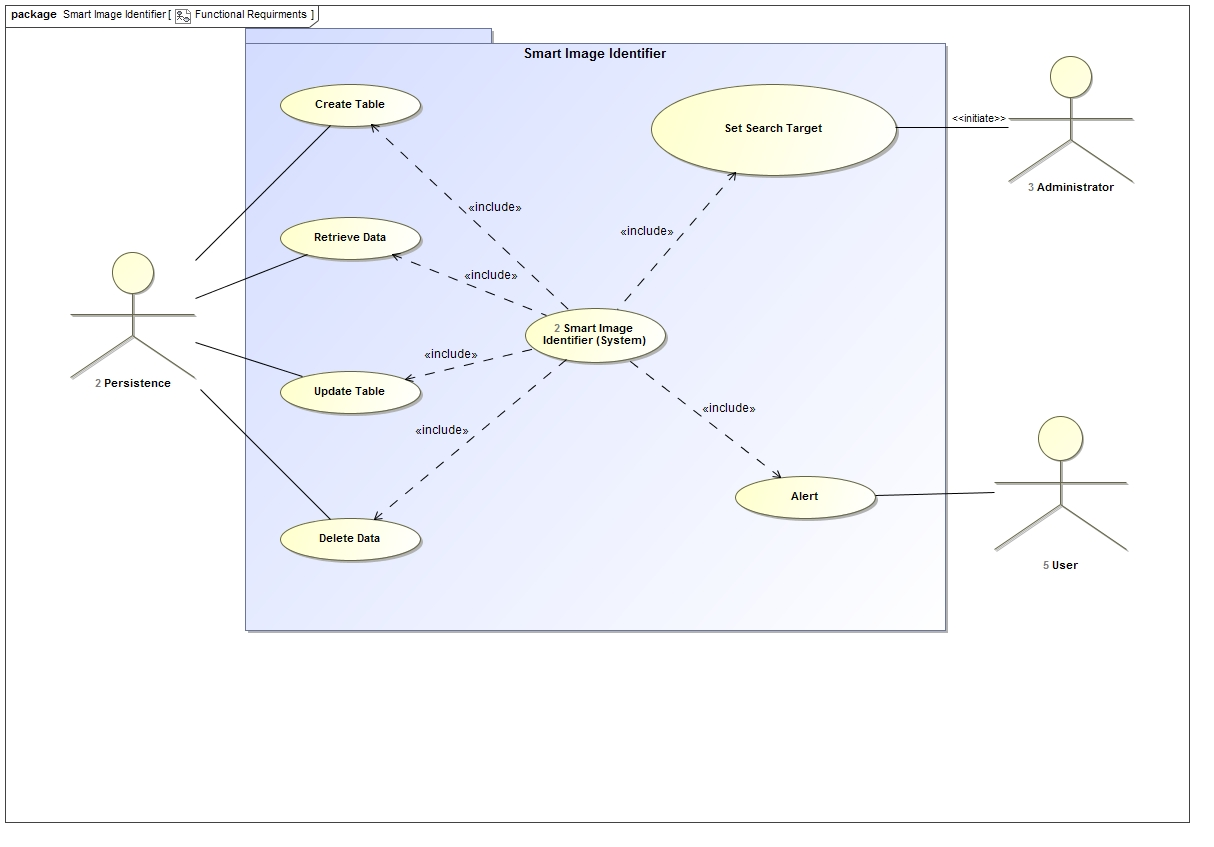
\includegraphics[width=1\textwidth]{./FunctionalRequirments.jpg}\\[1.5cm]
\end{document}